\documentclass[11pt]{article}
\usepackage[textwidth=18.0cm, textheight=23.0cm, top=2.0cm]{geometry}
\usepackage{pst-all}
\usepackage{amssymb}
\usepackage{tikz}
\usepackage{underscore}\begin{document}
\pagestyle{empty}


ClassName: \underline{\textbf{Class_05.2bp-19}}
\par
BinSize: \underline{\textbf{100 × 100}}
\par
ReduceSize: \underline{\textbf{100 × 100}}
\par
TypeNum: \underline{\textbf{40}}
\par
Num: \underline{\textbf{40}}
\par
OutS: \underline{\textbf{100000}}
\par
InS: \underline{\textbf{84528}}
\par
Rate: \underline{\textbf{0.845}}
\par
UB: \underline{\textbf{10}}
\par
LB0: \underline{\textbf{10}}
\par
LB: \underline{\textbf{10}}
\par
LBWithCut: \underline{\textbf{10}}
\par
NodeCut: \underline{\textbf{0}}
\par
ExtendedNodeCnt: \underline{\textbf{1}}
\par
GenNodeCnt: \underline{\textbf{1}}
\par
PrimalNode: \underline{\textbf{0}}
\par
ColumnCount: \underline{\textbf{10}}
\par
TotalCutCount: \underline{\textbf{0}}
\par
RootCutCount: \underline{\textbf{0}}
\par
LPSolverCnt: \underline{\textbf{1}}
\par
PricingSolverCnt: \underline{\textbf{0}}
\par
BranchAndBoundNum: \underline{\textbf{1}}
\par
isOpt: \underline{\textbf{true}}
\par
TimeOnInitSolution: \underline{\textbf{600.000 s}}
\par
TimeOnPrimal: \underline{\textbf{0.000 s}}
\par
TimeOnPricing: \underline{\textbf{0.000 s}}
\par
TimeOnRmp: \underline{\textbf{0.078 s}}
\par
TotalTime: \underline{\textbf{600.375 s}}
\par
\newpage


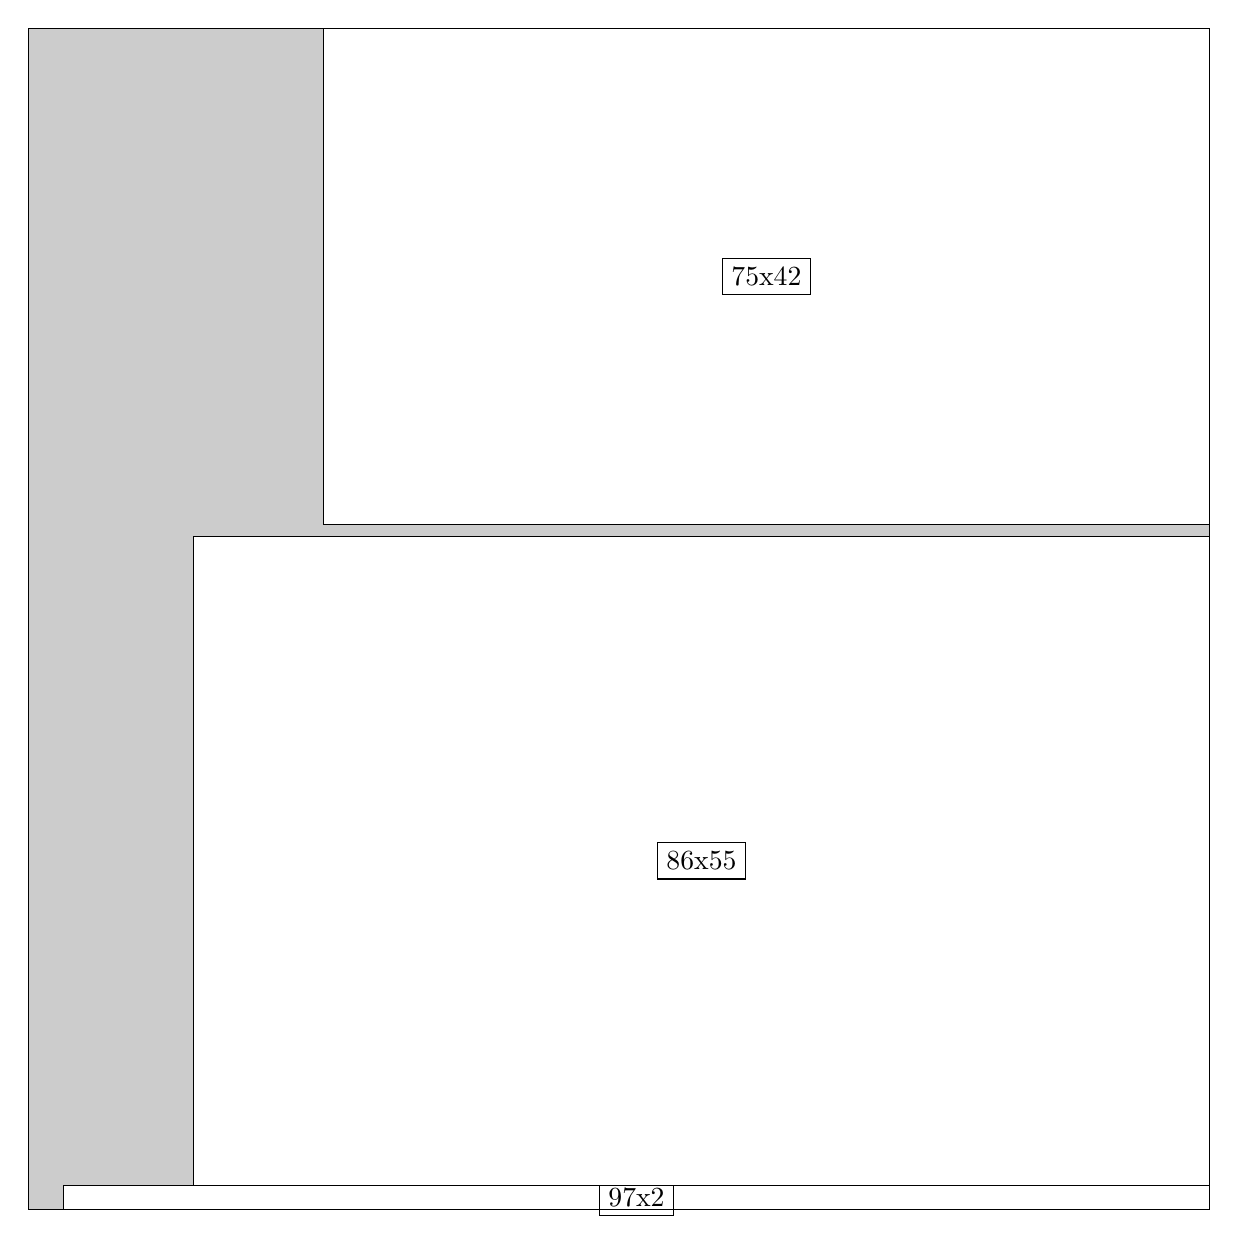
\begin{tikzpicture}[shorten >=1pt,scale=1.0,every node/.style={scale=1.0},->]
\tikzstyle{vertex}=[circle,fill=black!25,minimum size=14pt,inner sep=0pt]
\filldraw[fill=gray!40!white, draw=black] (0,0) rectangle (15.0,15.0);
\foreach \name/\x/\y/\w/\h in {97x2/0.44999999999999996/0.0/14.549999999999999/0.3,86x55/2.1/0.3/12.9/8.25,75x42/3.75/8.7/11.25/6.3}
\filldraw[fill=white!40!white, draw=black] (\x,\y) rectangle node[draw] (\name) {\name} ++(\w,\h);
\end{tikzpicture}


w =97 , h =2 , x =3 , y =0 , v =194
\par
w =86 , h =55 , x =14 , y =2 , v =4730
\par
w =75 , h =42 , x =25 , y =58 , v =3150
\par
\newpage


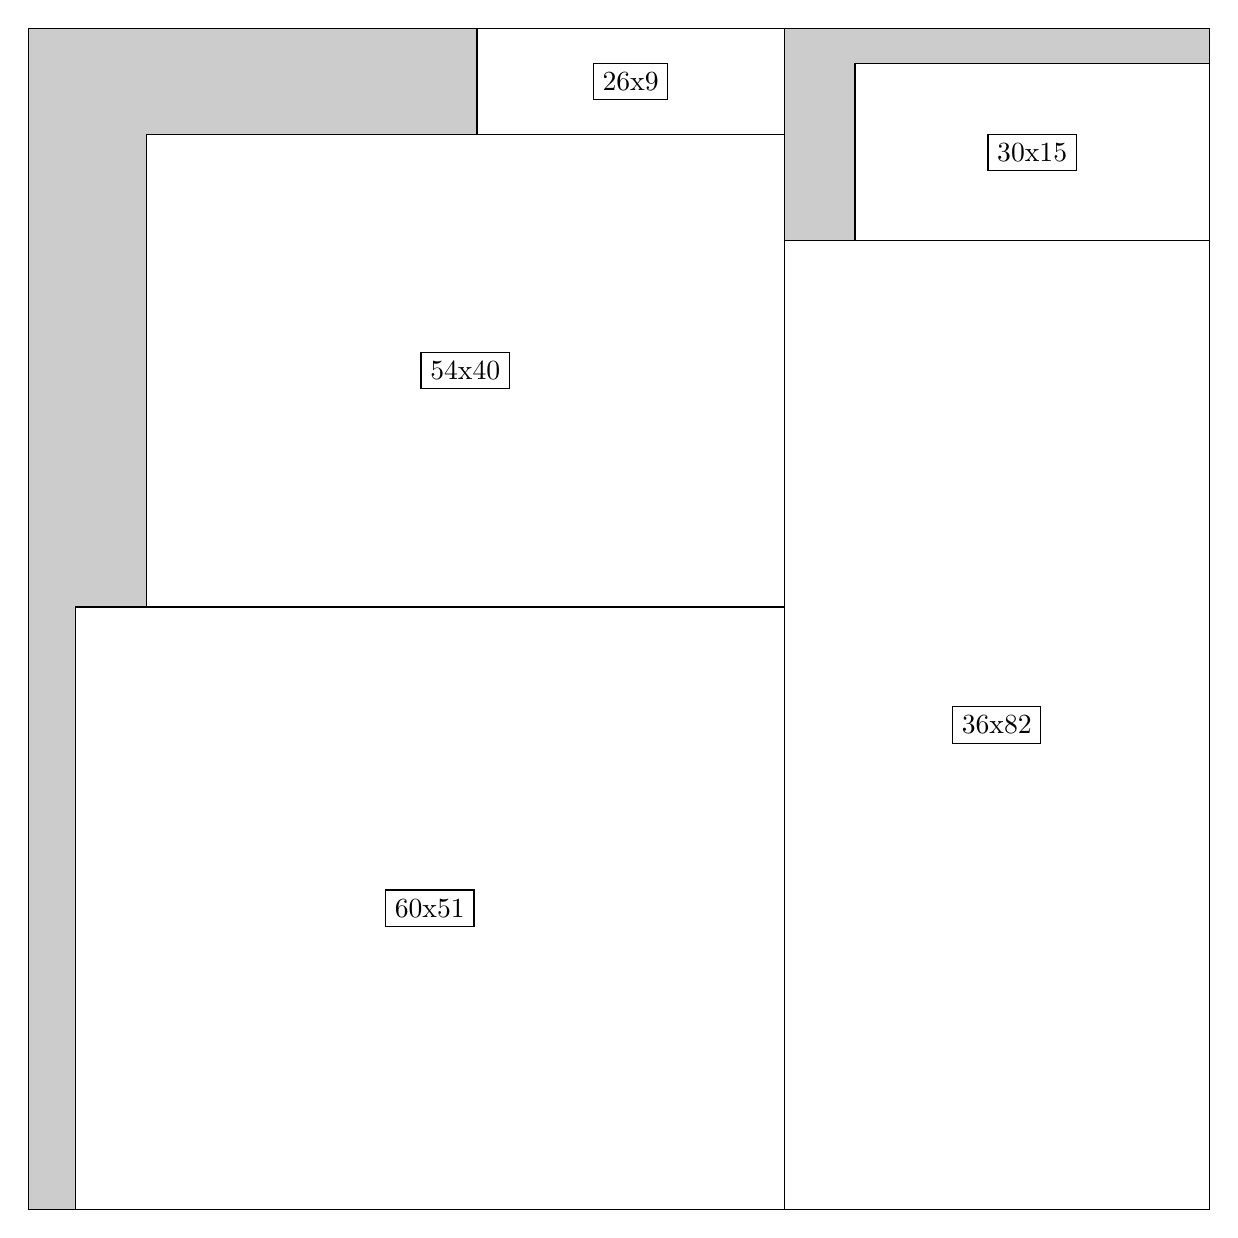
\begin{tikzpicture}[shorten >=1pt,scale=1.0,every node/.style={scale=1.0},->]
\tikzstyle{vertex}=[circle,fill=black!25,minimum size=14pt,inner sep=0pt]
\filldraw[fill=gray!40!white, draw=black] (0,0) rectangle (15.0,15.0);
\foreach \name/\x/\y/\w/\h in {36x82/9.6/0.0/5.3999999999999995/12.299999999999999,30x15/10.5/12.299999999999999/4.5/2.25,60x51/0.6/0.0/9.0/7.6499999999999995,54x40/1.5/7.6499999999999995/8.1/6.0,26x9/5.7/13.65/3.9/1.3499999999999999}
\filldraw[fill=white!40!white, draw=black] (\x,\y) rectangle node[draw] (\name) {\name} ++(\w,\h);
\end{tikzpicture}


w =36 , h =82 , x =64 , y =0 , v =2952
\par
w =30 , h =15 , x =70 , y =82 , v =450
\par
w =60 , h =51 , x =4 , y =0 , v =3060
\par
w =54 , h =40 , x =10 , y =51 , v =2160
\par
w =26 , h =9 , x =38 , y =91 , v =234
\par
\newpage


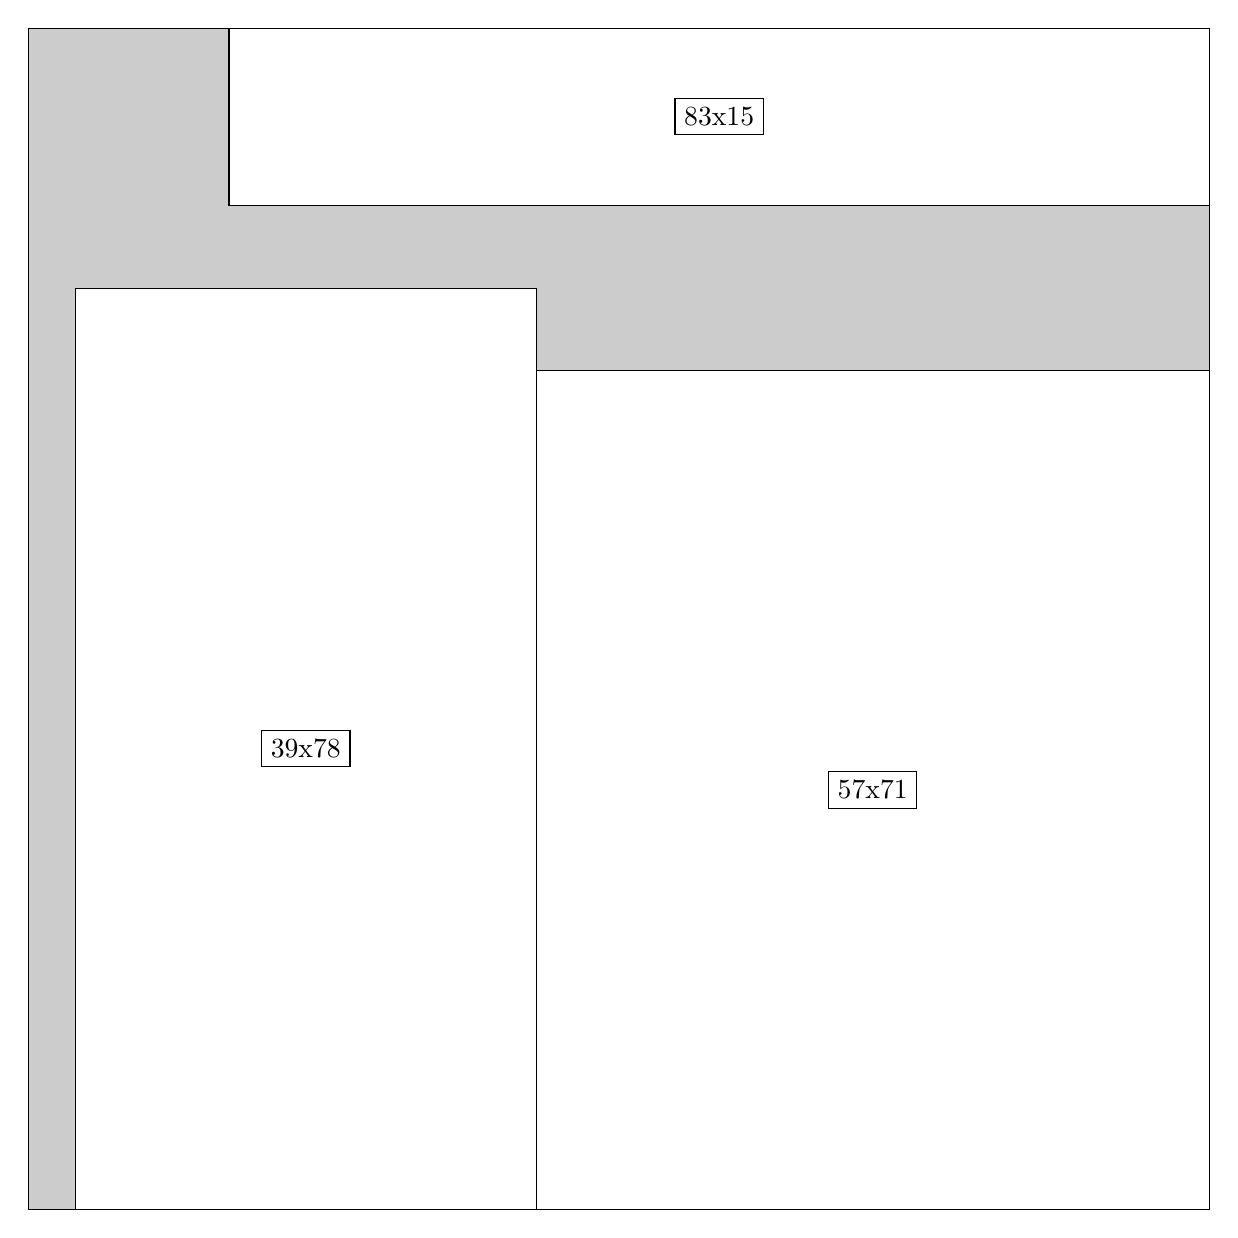
\begin{tikzpicture}[shorten >=1pt,scale=1.0,every node/.style={scale=1.0},->]
\tikzstyle{vertex}=[circle,fill=black!25,minimum size=14pt,inner sep=0pt]
\filldraw[fill=gray!40!white, draw=black] (0,0) rectangle (15.0,15.0);
\foreach \name/\x/\y/\w/\h in {57x71/6.45/0.0/8.549999999999999/10.65,39x78/0.6/0.0/5.85/11.7,83x15/2.55/12.75/12.45/2.25}
\filldraw[fill=white!40!white, draw=black] (\x,\y) rectangle node[draw] (\name) {\name} ++(\w,\h);
\end{tikzpicture}


w =57 , h =71 , x =43 , y =0 , v =4047
\par
w =39 , h =78 , x =4 , y =0 , v =3042
\par
w =83 , h =15 , x =17 , y =85 , v =1245
\par
\newpage


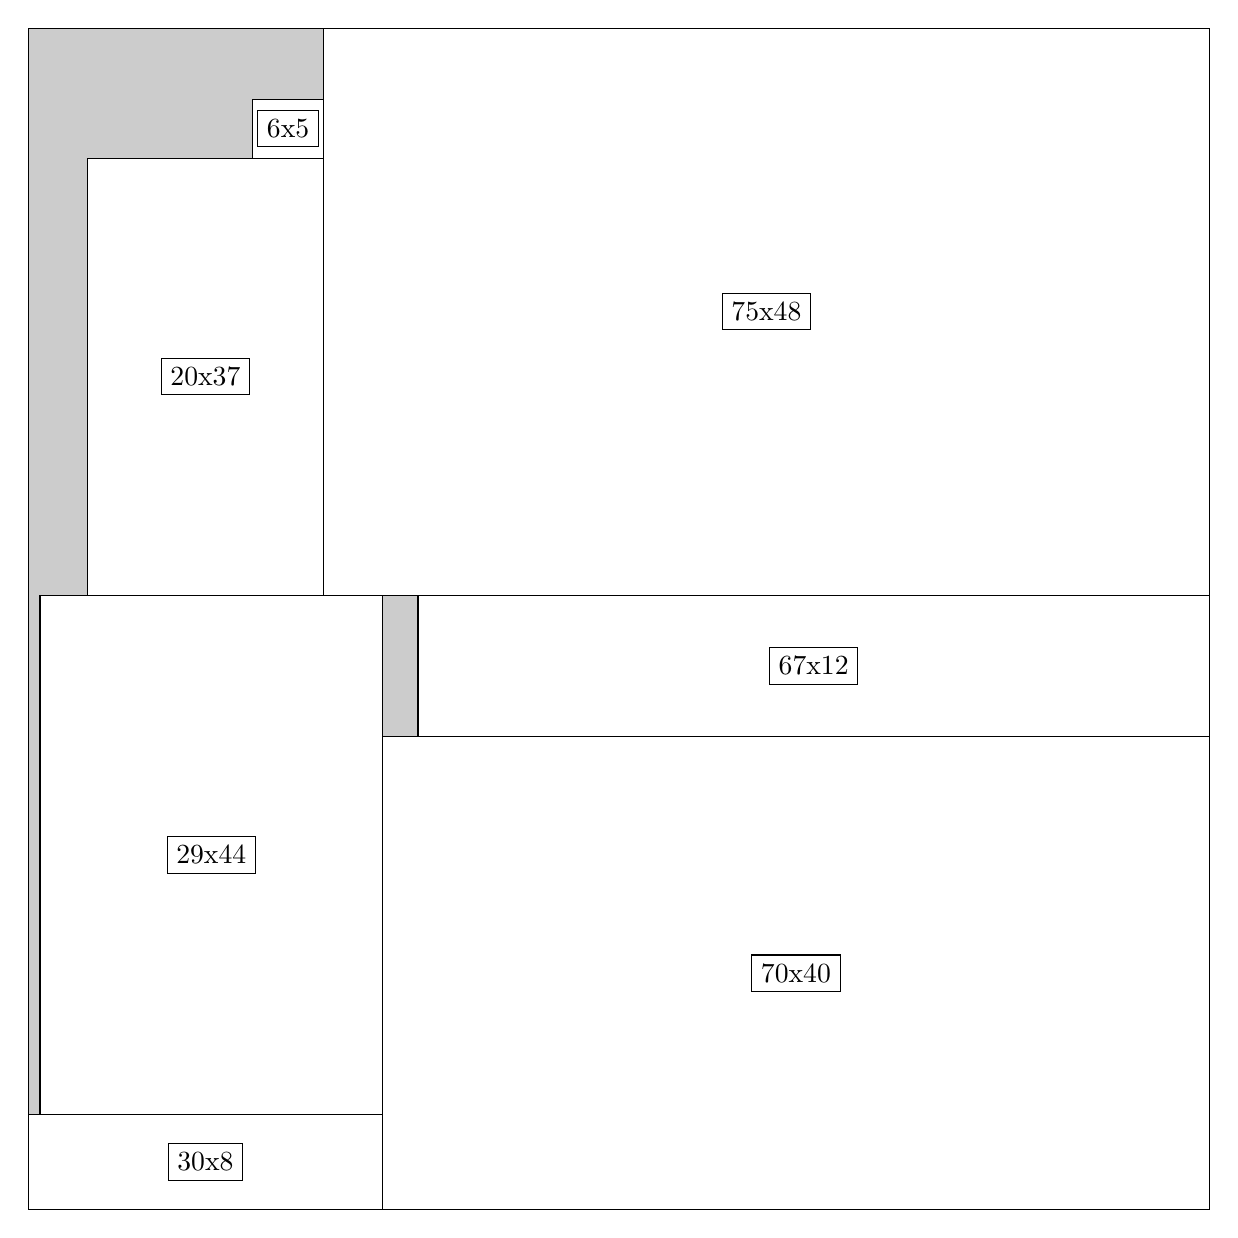
\begin{tikzpicture}[shorten >=1pt,scale=1.0,every node/.style={scale=1.0},->]
\tikzstyle{vertex}=[circle,fill=black!25,minimum size=14pt,inner sep=0pt]
\filldraw[fill=gray!40!white, draw=black] (0,0) rectangle (15.0,15.0);
\foreach \name/\x/\y/\w/\h in {70x40/4.5/0.0/10.5/6.0,67x12/4.95/6.0/10.049999999999999/1.7999999999999998,30x8/0.0/0.0/4.5/1.2,29x44/0.15/1.2/4.35/6.6,75x48/3.75/7.8/11.25/7.199999999999999,20x37/0.75/7.8/3.0/5.55,6x5/2.85/13.35/0.8999999999999999/0.75}
\filldraw[fill=white!40!white, draw=black] (\x,\y) rectangle node[draw] (\name) {\name} ++(\w,\h);
\end{tikzpicture}


w =70 , h =40 , x =30 , y =0 , v =2800
\par
w =67 , h =12 , x =33 , y =40 , v =804
\par
w =30 , h =8 , x =0 , y =0 , v =240
\par
w =29 , h =44 , x =1 , y =8 , v =1276
\par
w =75 , h =48 , x =25 , y =52 , v =3600
\par
w =20 , h =37 , x =5 , y =52 , v =740
\par
w =6 , h =5 , x =19 , y =89 , v =30
\par
\newpage


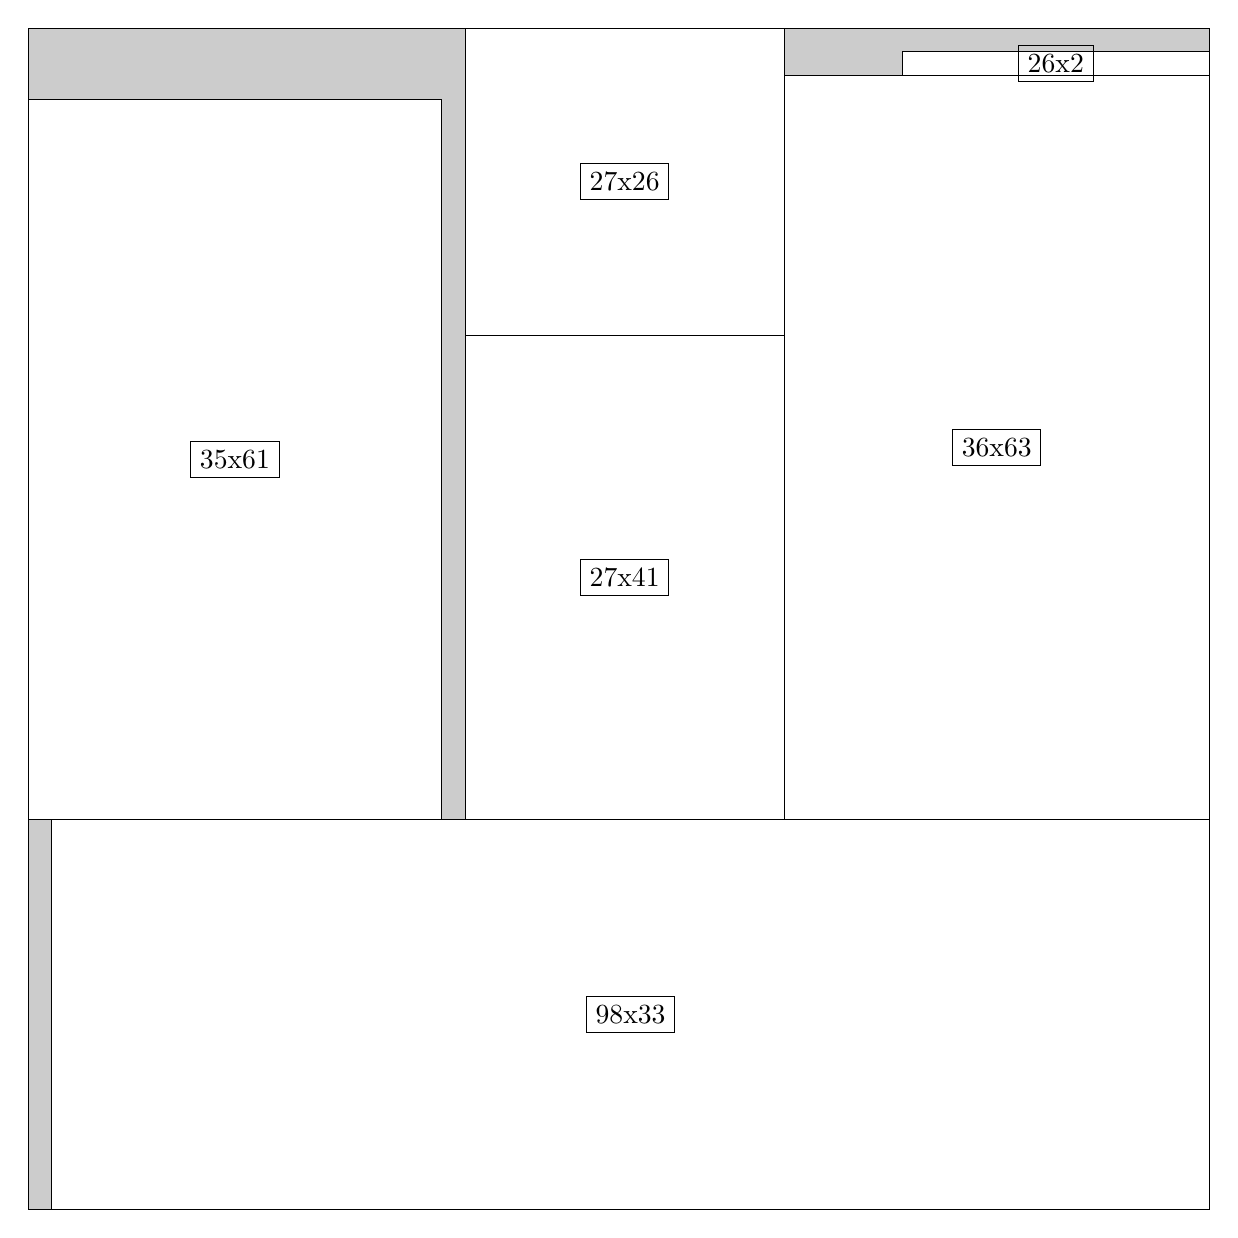
\begin{tikzpicture}[shorten >=1pt,scale=1.0,every node/.style={scale=1.0},->]
\tikzstyle{vertex}=[circle,fill=black!25,minimum size=14pt,inner sep=0pt]
\filldraw[fill=gray!40!white, draw=black] (0,0) rectangle (15.0,15.0);
\foreach \name/\x/\y/\w/\h in {98x33/0.3/0.0/14.7/4.95,36x63/9.6/4.95/5.3999999999999995/9.45,26x2/11.1/14.399999999999999/3.9/0.3,27x41/5.55/4.95/4.05/6.1499999999999995,27x26/5.55/11.1/4.05/3.9,35x61/0.0/4.95/5.25/9.15}
\filldraw[fill=white!40!white, draw=black] (\x,\y) rectangle node[draw] (\name) {\name} ++(\w,\h);
\end{tikzpicture}


w =98 , h =33 , x =2 , y =0 , v =3234
\par
w =36 , h =63 , x =64 , y =33 , v =2268
\par
w =26 , h =2 , x =74 , y =96 , v =52
\par
w =27 , h =41 , x =37 , y =33 , v =1107
\par
w =27 , h =26 , x =37 , y =74 , v =702
\par
w =35 , h =61 , x =0 , y =33 , v =2135
\par
\newpage


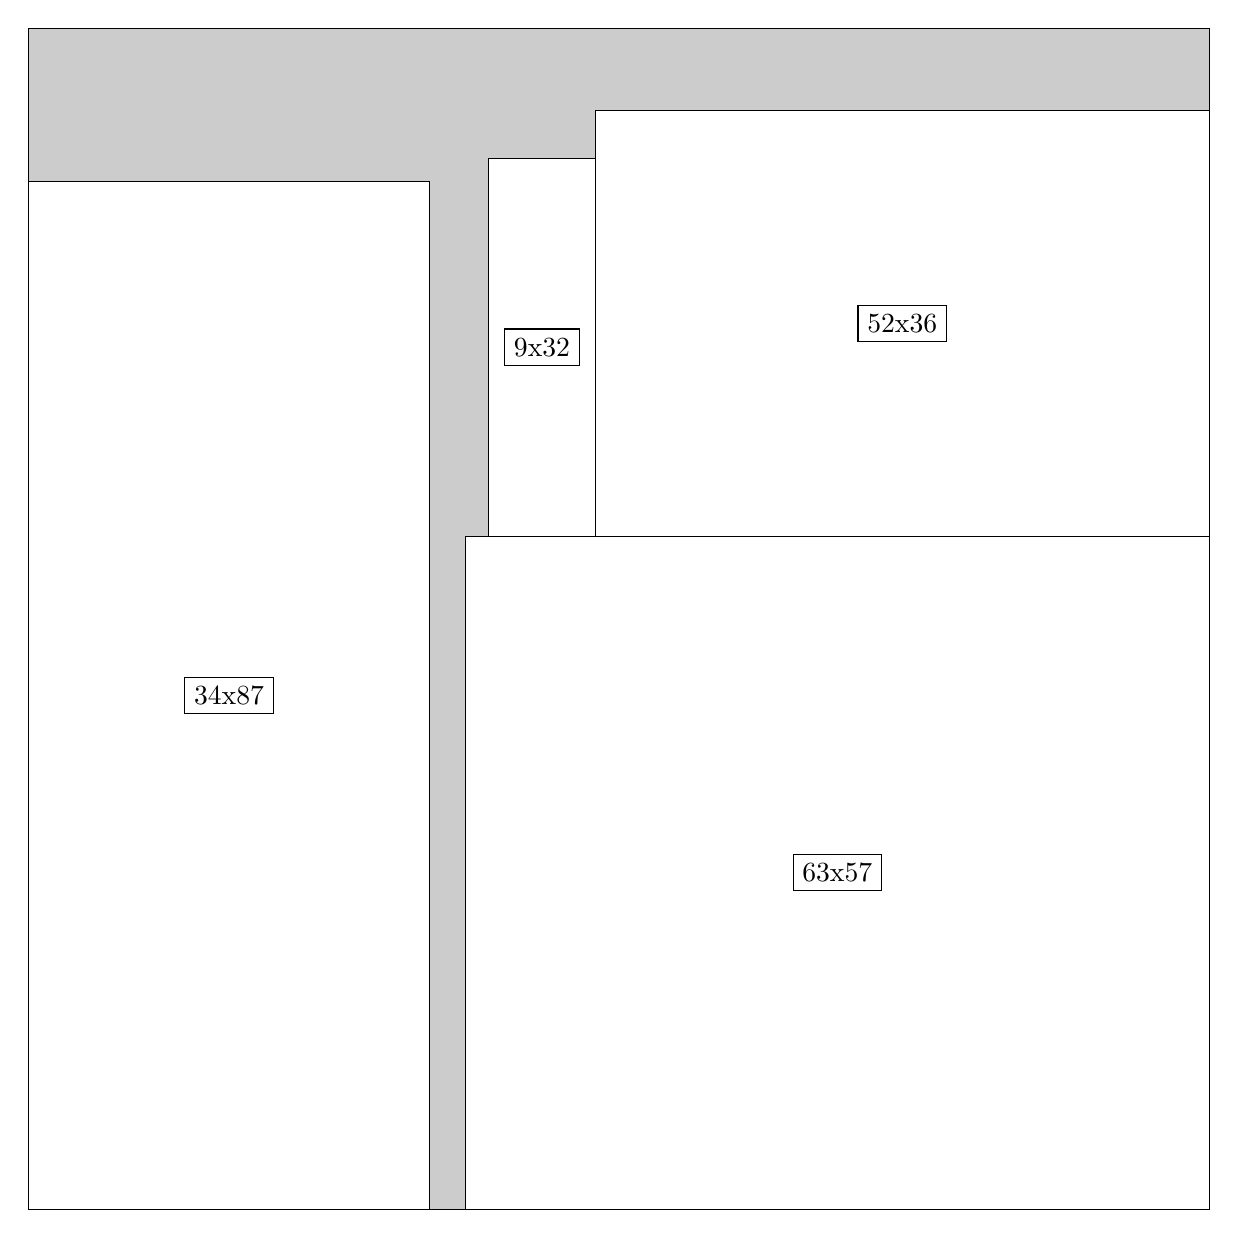
\begin{tikzpicture}[shorten >=1pt,scale=1.0,every node/.style={scale=1.0},->]
\tikzstyle{vertex}=[circle,fill=black!25,minimum size=14pt,inner sep=0pt]
\filldraw[fill=gray!40!white, draw=black] (0,0) rectangle (15.0,15.0);
\foreach \name/\x/\y/\w/\h in {63x57/5.55/0.0/9.45/8.549999999999999,52x36/7.199999999999999/8.549999999999999/7.8/5.3999999999999995,9x32/5.85/8.549999999999999/1.3499999999999999/4.8,34x87/0.0/0.0/5.1/13.049999999999999}
\filldraw[fill=white!40!white, draw=black] (\x,\y) rectangle node[draw] (\name) {\name} ++(\w,\h);
\end{tikzpicture}


w =63 , h =57 , x =37 , y =0 , v =3591
\par
w =52 , h =36 , x =48 , y =57 , v =1872
\par
w =9 , h =32 , x =39 , y =57 , v =288
\par
w =34 , h =87 , x =0 , y =0 , v =2958
\par
\newpage


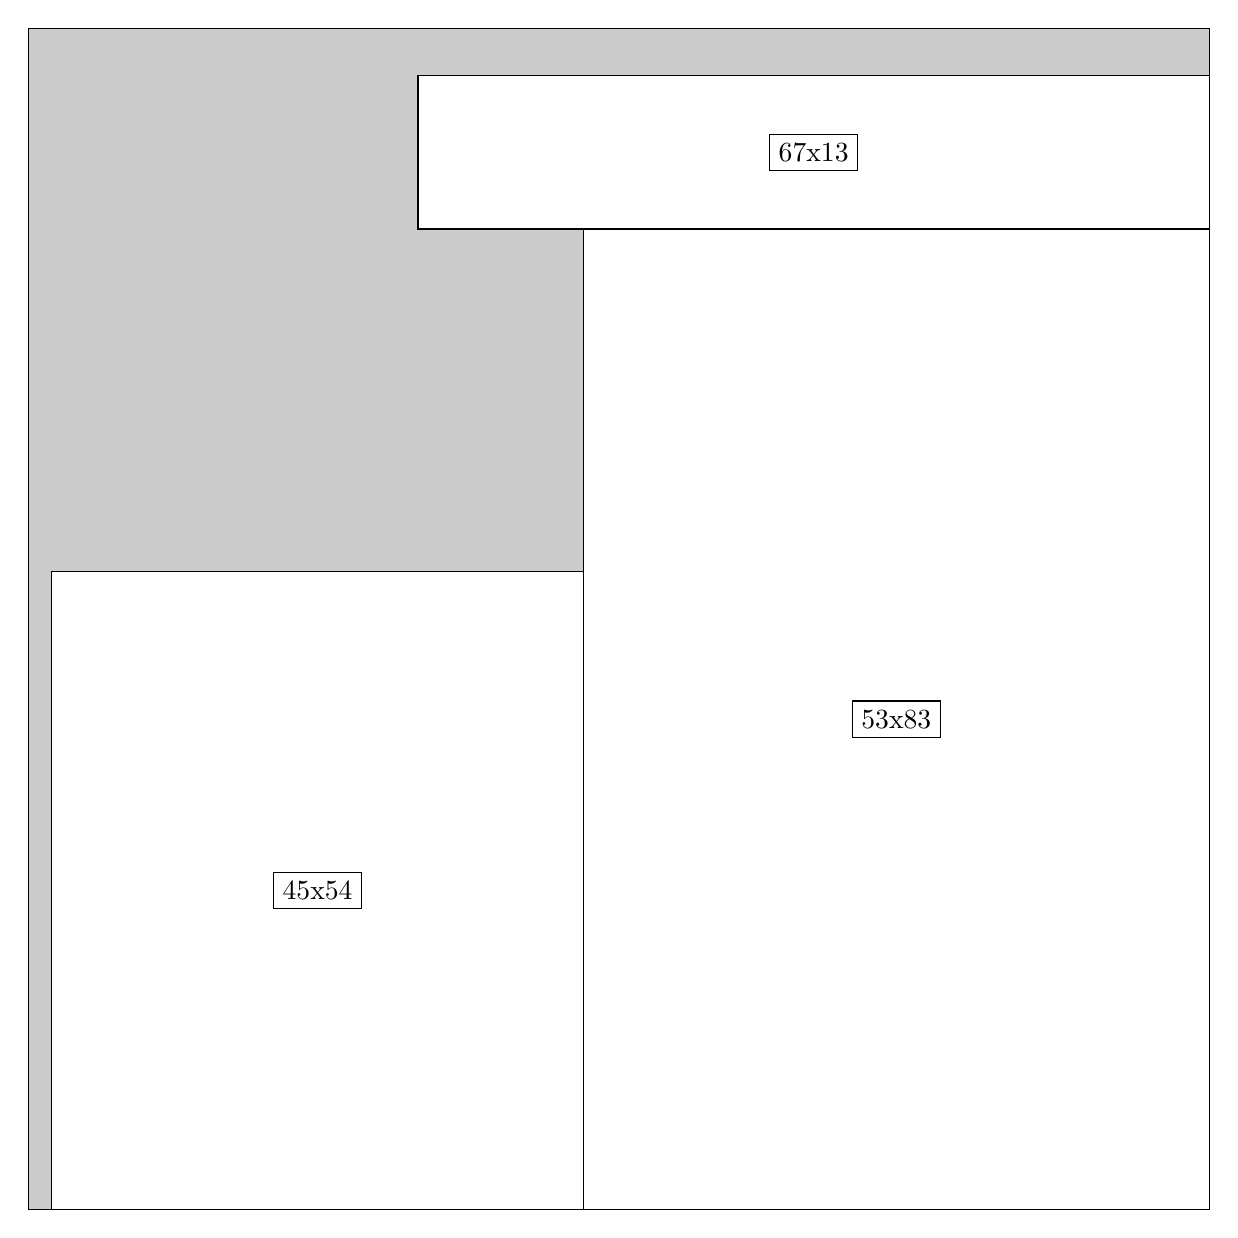
\begin{tikzpicture}[shorten >=1pt,scale=1.0,every node/.style={scale=1.0},->]
\tikzstyle{vertex}=[circle,fill=black!25,minimum size=14pt,inner sep=0pt]
\filldraw[fill=gray!40!white, draw=black] (0,0) rectangle (15.0,15.0);
\foreach \name/\x/\y/\w/\h in {53x83/7.05/0.0/7.949999999999999/12.45,45x54/0.3/0.0/6.75/8.1,67x13/4.95/12.45/10.049999999999999/1.95}
\filldraw[fill=white!40!white, draw=black] (\x,\y) rectangle node[draw] (\name) {\name} ++(\w,\h);
\end{tikzpicture}


w =53 , h =83 , x =47 , y =0 , v =4399
\par
w =45 , h =54 , x =2 , y =0 , v =2430
\par
w =67 , h =13 , x =33 , y =83 , v =871
\par
\newpage


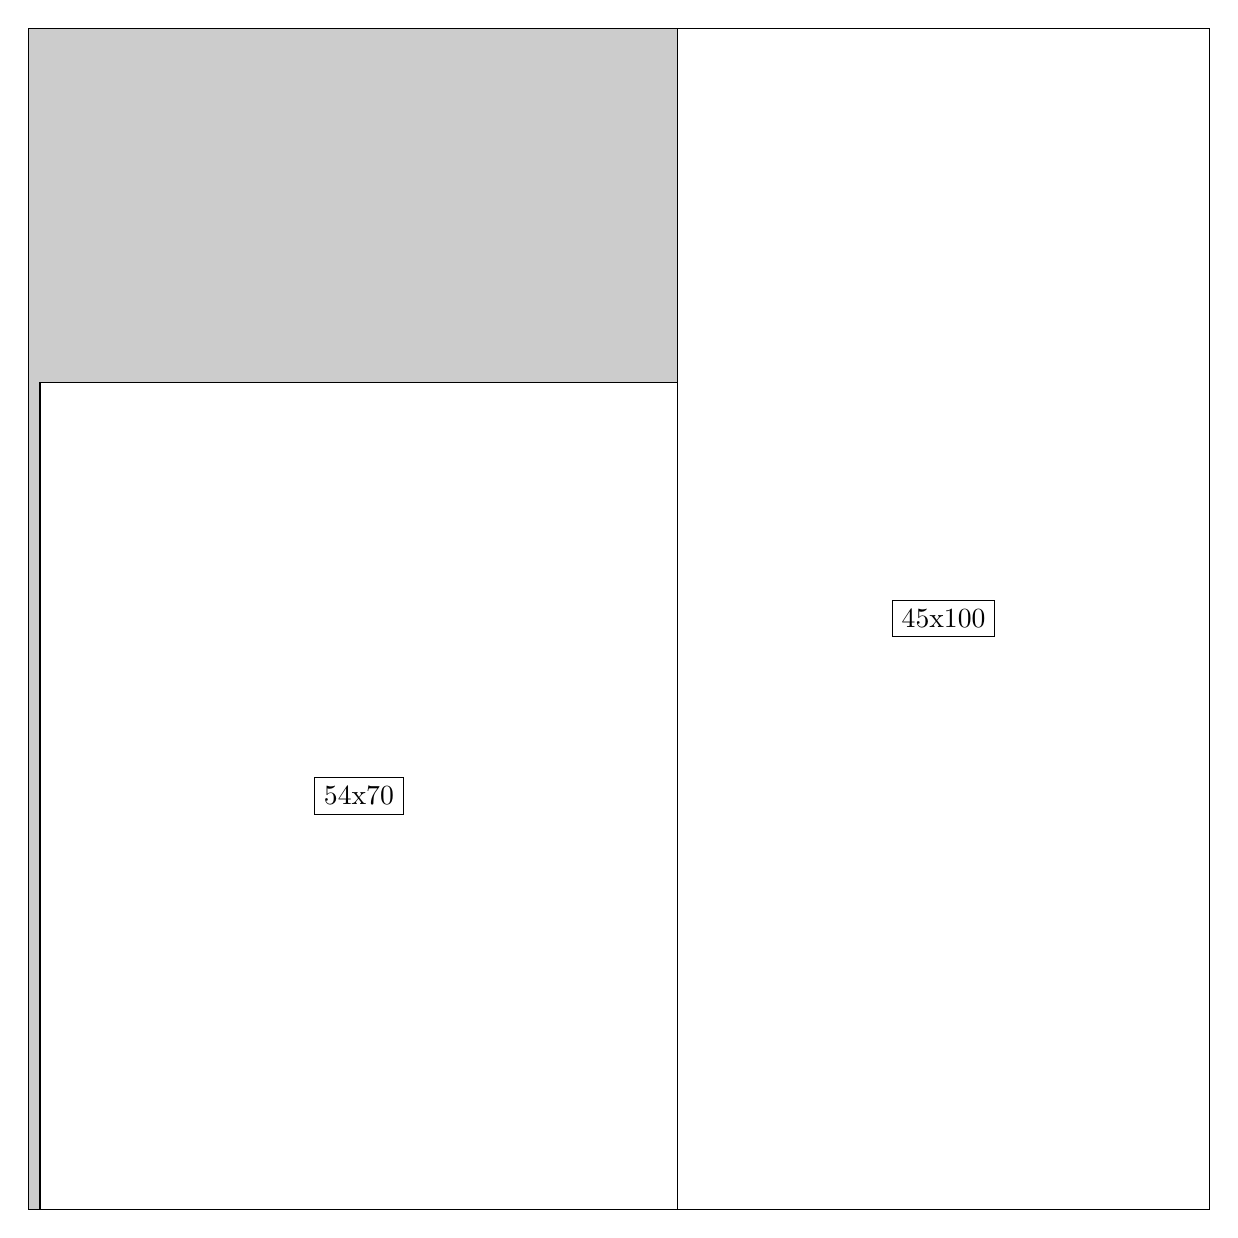
\begin{tikzpicture}[shorten >=1pt,scale=1.0,every node/.style={scale=1.0},->]
\tikzstyle{vertex}=[circle,fill=black!25,minimum size=14pt,inner sep=0pt]
\filldraw[fill=gray!40!white, draw=black] (0,0) rectangle (15.0,15.0);
\foreach \name/\x/\y/\w/\h in {45x100/8.25/0.0/6.75/15.0,54x70/0.15/0.0/8.1/10.5}
\filldraw[fill=white!40!white, draw=black] (\x,\y) rectangle node[draw] (\name) {\name} ++(\w,\h);
\end{tikzpicture}


w =45 , h =100 , x =55 , y =0 , v =4500
\par
w =54 , h =70 , x =1 , y =0 , v =3780
\par
\newpage


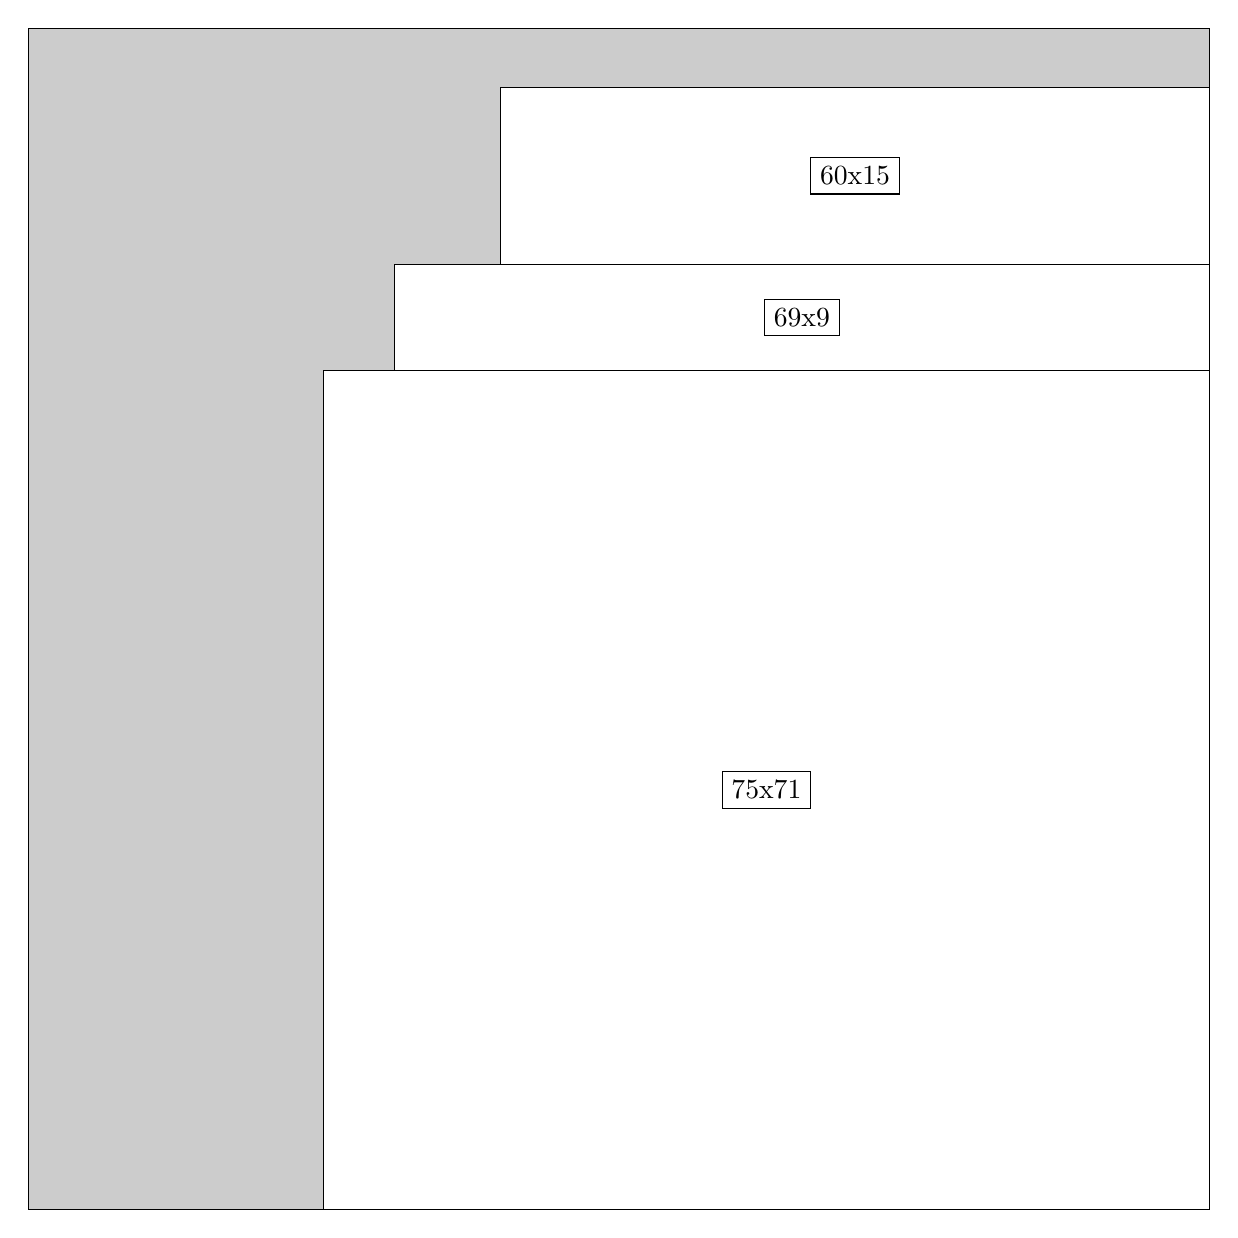
\begin{tikzpicture}[shorten >=1pt,scale=1.0,every node/.style={scale=1.0},->]
\tikzstyle{vertex}=[circle,fill=black!25,minimum size=14pt,inner sep=0pt]
\filldraw[fill=gray!40!white, draw=black] (0,0) rectangle (15.0,15.0);
\foreach \name/\x/\y/\w/\h in {75x71/3.75/0.0/11.25/10.65,69x9/4.6499999999999995/10.65/10.35/1.3499999999999999,60x15/6.0/12.0/9.0/2.25}
\filldraw[fill=white!40!white, draw=black] (\x,\y) rectangle node[draw] (\name) {\name} ++(\w,\h);
\end{tikzpicture}


w =75 , h =71 , x =25 , y =0 , v =5325
\par
w =69 , h =9 , x =31 , y =71 , v =621
\par
w =60 , h =15 , x =40 , y =80 , v =900
\par
\newpage


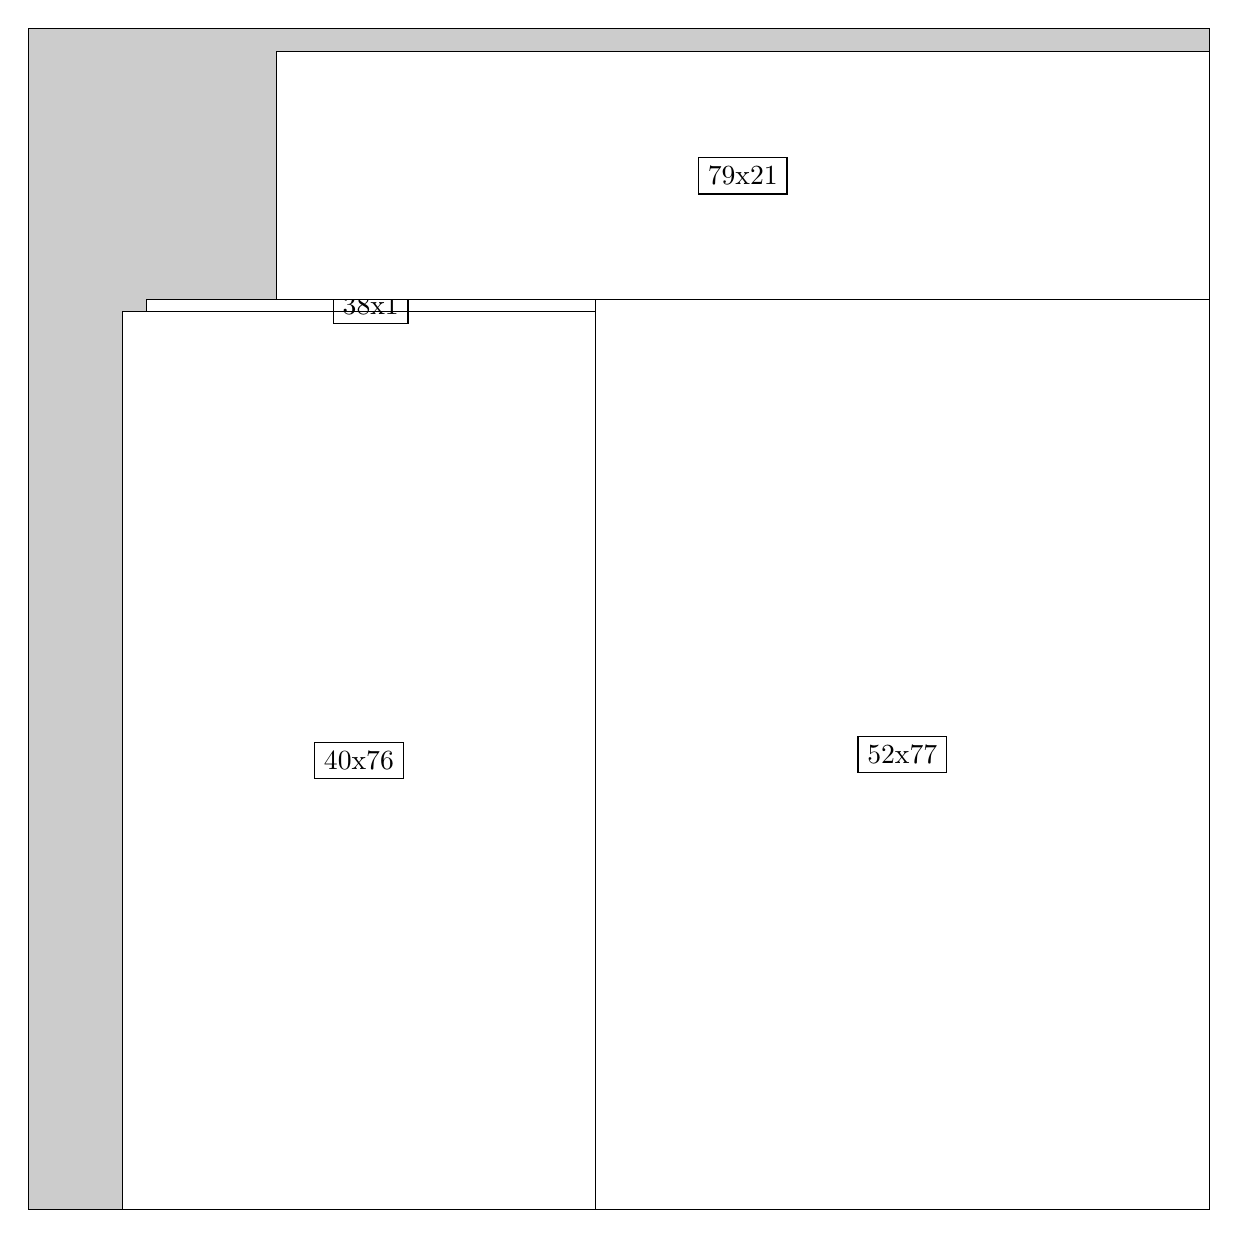
\begin{tikzpicture}[shorten >=1pt,scale=1.0,every node/.style={scale=1.0},->]
\tikzstyle{vertex}=[circle,fill=black!25,minimum size=14pt,inner sep=0pt]
\filldraw[fill=gray!40!white, draw=black] (0,0) rectangle (15.0,15.0);
\foreach \name/\x/\y/\w/\h in {52x77/7.199999999999999/0.0/7.8/11.549999999999999,40x76/1.2/0.0/6.0/11.4,38x1/1.5/11.4/5.7/0.15,79x21/3.15/11.549999999999999/11.85/3.15}
\filldraw[fill=white!40!white, draw=black] (\x,\y) rectangle node[draw] (\name) {\name} ++(\w,\h);
\end{tikzpicture}


w =52 , h =77 , x =48 , y =0 , v =4004
\par
w =40 , h =76 , x =8 , y =0 , v =3040
\par
w =38 , h =1 , x =10 , y =76 , v =38
\par
w =79 , h =21 , x =21 , y =77 , v =1659
\par
\newpage


\end{document}